% Options for packages loaded elsewhere
% Options for packages loaded elsewhere
\PassOptionsToPackage{unicode}{hyperref}
\PassOptionsToPackage{hyphens}{url}
\PassOptionsToPackage{dvipsnames,svgnames,x11names}{xcolor}
%
\documentclass[
  british,
  a4paper,
]{article}
\usepackage{xcolor}
\usepackage{amsmath,amssymb}
\setcounter{secnumdepth}{-\maxdimen} % remove section numbering
\usepackage{iftex}
\ifPDFTeX
  \usepackage[T1]{fontenc}
  \usepackage[utf8]{inputenc}
  \usepackage{textcomp} % provide euro and other symbols
\else % if luatex or xetex
  \usepackage{unicode-math} % this also loads fontspec
  \defaultfontfeatures{Scale=MatchLowercase}
  \defaultfontfeatures[\rmfamily]{Ligatures=TeX,Scale=1}
\fi
\usepackage{lmodern}
\ifPDFTeX\else
  % xetex/luatex font selection
\fi
% Use upquote if available, for straight quotes in verbatim environments
\IfFileExists{upquote.sty}{\usepackage{upquote}}{}
\IfFileExists{microtype.sty}{% use microtype if available
  \usepackage[]{microtype}
  \UseMicrotypeSet[protrusion]{basicmath} % disable protrusion for tt fonts
}{}
\makeatletter
\@ifundefined{KOMAClassName}{% if non-KOMA class
  \IfFileExists{parskip.sty}{%
    \usepackage{parskip}
  }{% else
    \setlength{\parindent}{0pt}
    \setlength{\parskip}{6pt plus 2pt minus 1pt}}
}{% if KOMA class
  \KOMAoptions{parskip=half}}
\makeatother
% Make \paragraph and \subparagraph free-standing
\makeatletter
\ifx\paragraph\undefined\else
  \let\oldparagraph\paragraph
  \renewcommand{\paragraph}{
    \@ifstar
      \xxxParagraphStar
      \xxxParagraphNoStar
  }
  \newcommand{\xxxParagraphStar}[1]{\oldparagraph*{#1}\mbox{}}
  \newcommand{\xxxParagraphNoStar}[1]{\oldparagraph{#1}\mbox{}}
\fi
\ifx\subparagraph\undefined\else
  \let\oldsubparagraph\subparagraph
  \renewcommand{\subparagraph}{
    \@ifstar
      \xxxSubParagraphStar
      \xxxSubParagraphNoStar
  }
  \newcommand{\xxxSubParagraphStar}[1]{\oldsubparagraph*{#1}\mbox{}}
  \newcommand{\xxxSubParagraphNoStar}[1]{\oldsubparagraph{#1}\mbox{}}
\fi
\makeatother


\usepackage{longtable,booktabs,array}
\newcounter{none} % for unnumbered tables
\usepackage{calc} % for calculating minipage widths
% Correct order of tables after \paragraph or \subparagraph
\usepackage{etoolbox}
\makeatletter
\patchcmd\longtable{\par}{\if@noskipsec\mbox{}\fi\par}{}{}
\makeatother
% Allow footnotes in longtable head/foot
\IfFileExists{footnotehyper.sty}{\usepackage{footnotehyper}}{\usepackage{footnote}}
\makesavenoteenv{longtable}
\usepackage{graphicx}
\makeatletter
\newsavebox\pandoc@box
\newcommand*\pandocbounded[1]{% scales image to fit in text height/width
  \sbox\pandoc@box{#1}%
  \Gscale@div\@tempa{\textheight}{\dimexpr\ht\pandoc@box+\dp\pandoc@box\relax}%
  \Gscale@div\@tempb{\linewidth}{\wd\pandoc@box}%
  \ifdim\@tempb\p@<\@tempa\p@\let\@tempa\@tempb\fi% select the smaller of both
  \ifdim\@tempa\p@<\p@\scalebox{\@tempa}{\usebox\pandoc@box}%
  \else\usebox{\pandoc@box}%
  \fi%
}
% Set default figure placement to htbp
\def\fps@figure{htbp}
\makeatother



\ifLuaTeX
\usepackage[bidi=basic,shorthands=off]{babel}
\else
\usepackage[bidi=default,shorthands=off]{babel}
\fi
\ifLuaTeX
  \usepackage{selnolig} % disable illegal ligatures
\fi


\setlength{\emergencystretch}{3em} % prevent overfull lines

\providecommand{\tightlist}{%
  \setlength{\itemsep}{0pt}\setlength{\parskip}{0pt}}



 


\makeatletter
\@ifpackageloaded{tcolorbox}{}{\usepackage[skins,breakable]{tcolorbox}}
\@ifpackageloaded{fontawesome5}{}{\usepackage{fontawesome5}}
\definecolor{quarto-callout-color}{HTML}{909090}
\definecolor{quarto-callout-note-color}{HTML}{0758E5}
\definecolor{quarto-callout-important-color}{HTML}{CC1914}
\definecolor{quarto-callout-warning-color}{HTML}{EB9113}
\definecolor{quarto-callout-tip-color}{HTML}{00A047}
\definecolor{quarto-callout-caution-color}{HTML}{FC5300}
\definecolor{quarto-callout-color-frame}{HTML}{acacac}
\definecolor{quarto-callout-note-color-frame}{HTML}{4582ec}
\definecolor{quarto-callout-important-color-frame}{HTML}{d9534f}
\definecolor{quarto-callout-warning-color-frame}{HTML}{f0ad4e}
\definecolor{quarto-callout-tip-color-frame}{HTML}{02b875}
\definecolor{quarto-callout-caution-color-frame}{HTML}{fd7e14}
\makeatother
\makeatletter
\@ifpackageloaded{caption}{}{\usepackage{caption}}
\AtBeginDocument{%
\ifdefined\contentsname
  \renewcommand*\contentsname{Table of contents}
\else
  \newcommand\contentsname{Table of contents}
\fi
\ifdefined\listfigurename
  \renewcommand*\listfigurename{List of Figures}
\else
  \newcommand\listfigurename{List of Figures}
\fi
\ifdefined\listtablename
  \renewcommand*\listtablename{List of Tables}
\else
  \newcommand\listtablename{List of Tables}
\fi
\ifdefined\figurename
  \renewcommand*\figurename{Figure}
\else
  \newcommand\figurename{Figure}
\fi
\ifdefined\tablename
  \renewcommand*\tablename{Table}
\else
  \newcommand\tablename{Table}
\fi
}
\@ifpackageloaded{float}{}{\usepackage{float}}
\floatstyle{ruled}
\@ifundefined{c@chapter}{\newfloat{codelisting}{h}{lop}}{\newfloat{codelisting}{h}{lop}[chapter]}
\floatname{codelisting}{Listing}
\newcommand*\listoflistings{\listof{codelisting}{List of Listings}}
\makeatother
\makeatletter
\makeatother
\makeatletter
\@ifpackageloaded{caption}{}{\usepackage{caption}}
\@ifpackageloaded{subcaption}{}{\usepackage{subcaption}}
\makeatother
\usepackage{bookmark}
\IfFileExists{xurl.sty}{\usepackage{xurl}}{} % add URL line breaks if available
\urlstyle{same}
% fallback for those not using the hyperref driver hyperxmp:
\makeatletter
\@ifundefined{xmpquote}{\newcommand{\xmpquote}[1]{#1}}{}
\makeatother
\hypersetup{
  pdftitle={An automated feed for component-level US inflation},
  pdfauthor={Carlos Galindo},
  pdflang={en-GB},
  colorlinks=true,
  linkcolor={blue},
  filecolor={Maroon},
  citecolor={Blue},
  urlcolor={Blue},
  pdfcreator={LaTeX via pandoc}}


\title{An automated feed for component-level US inflation}
\usepackage{etoolbox}
\makeatletter
\providecommand{\subtitle}[1]{% add subtitle to \maketitle
  \apptocmd{\@title}{\par {\large #1 \par}}{}{}
}
\makeatother
\subtitle{A routine that pulls official price data, keeps it current and
turns it into monthly contributions to headline inflation}
\author{Carlos Galindo}
\date{}
\begin{document}
\maketitle


\begin{tcolorbox}[enhanced jigsaw, arc=.35mm, bottomrule=.15mm, breakable, colback=white, colframe=quarto-callout-note-color-frame, left=2mm, leftrule=.75mm, opacityback=0, rightrule=.15mm, toprule=.15mm]

\vspace{-3mm}\textbf{At a glance}\vspace{3mm}

\begin{itemize}
\tightlist
\item
  \textbf{Question.} What is driving US consumer inflation this month,
  component by component, and can that answer be refreshed without
  manual work?
\item
  \textbf{Approach.} An automated feed from the official statistical
  agency, with change detection and revision handling, feeding a
  decomposition that turns each component's price change into a
  contribution to the headline rate.
\item
  \textbf{Finding.} The decomposition is built to add back to the
  published headline, and the remaining gap is logged every month as a
  quality check.
\item
  \textbf{Why it matters.} Bottom-up forecasting of inflation needs a
  clean, current, additive component dataset before any model can be
  fitted.
\end{itemize}

\end{tcolorbox}

\subsection{The question}\label{the-question}

Headline inflation is a weighted average of many price indices, from
food and rent to airfares and used cars. A forecaster who only watches
the headline sees that prices moved but not why. A bottom-up view asks
which components pushed the rate up or down, how persistent each push is
likely to be, and what that implies for the next print. Every one of
those questions starts from the same raw material: a complete, current
and consistent set of component price series, together with the weights
that say how much each component counts.

Assembling that material by hand is slow and error-prone. Downloads are
manual, the agency revises recent figures, new series appear, and the
expenditure weights are published once a year in a different form from
the prices. Between annual updates the effective weight of each
component drifts, because components whose prices rise faster than
average claim a growing share of the basket. A decomposition that
ignores this drift will not add up to the headline.

The project in 2025 was to replace that manual routine with an automated
feed that anyone doing component-level analysis could rely on.

\subsection{Approach}\label{approach}

\subsubsection{The data feed}\label{the-data-feed}

The feed draws monthly price indices for the whole published hierarchy
of US consumer prices, a catalogue of 183 series spanning the headline,
its groups and its components, from the statistical agency's public
programmatic interface. The history starts in January 2006 and runs to
the latest release. The design goals were that it should be cheap to
run, safe to repeat and honest about what it has and has not got.

\begin{itemize}
\tightlist
\item
  \textbf{Change detection first.} Before downloading anything, the
  routine asks for a small sentinel series, usually the headline, and
  compares its latest period with what is stored. If nothing is new it
  stops. A short-lived memory of recent checks avoids repeat requests
  inside the same working session.
\item
  \textbf{Incremental updates with a revision window.} When there is
  news, only a recent window is re-fetched, and it overwrites the stored
  values for those months. The window looks back twelve months and
  extends further early in the year, when seasonal factors are
  re-estimated and the agency revises more of the recent past.
\item
  \textbf{Strict failure rules.} A request that returns an empty or
  partial answer for any series aborts the update and leaves the stored
  base untouched, rather than writing a dataset with silent holes.
  Transient errors are retried with increasing delays and the agency's
  request limits are respected.
\item
  \textbf{Coverage checks.} A long history needs a registered access
  key. The routine checks that the span it received matches the span it
  asked for, so that a shortened history cannot pass unnoticed.
\item
  \textbf{A catalogue alongside the data.} Series titles and survey
  metadata are stored beside the numbers, so every component can be
  labelled and placed in the hierarchy.
\end{itemize}

\subsubsection{From prices to
contributions}\label{from-prices-to-contributions}

The second layer turns index levels into contributions. For each month
the routine takes the previous month's effective weight of every
lowest-level component, multiplies it by that component's monthly
percentage change, and records the result in percentage points. Summing
the components gives the headline change, and the same sums give every
intermediate group, such as food, energy, shelter or core goods.

The effective weights are rebuilt rather than read from a table. Each
December the agency publishes expenditure weights. The routine takes the
weights of the prior December and moves them forward month by month in
proportion to each component's relative price movement, then
renormalises, which is a Laspeyres-style approximation using prior-month
prices. Components are classified as leaves or aggregates from the
structure of their codes, and the headline is excluded from the leaves
so nothing is counted twice.

\subsubsection{Checking it}\label{checking-it}

The check is built into the output. Each month the routine stores the
residual, defined as the published headline change minus the sum of the
component contributions. A tolerance triggers a warning if the residual
is too large, and persistent residuals point to a specific cause:
components missing from the weight table, a mistaken place in the
hierarchy, or a normalisation problem. The weights are renormalised only
when the leaf total drifts by more than half a percentage point from one
hundred, so that rounding noise is not mistaken for a real discrepancy.

\subsection{What the work shows}\label{what-the-work-shows}

\subsubsection{An additive decomposition with a monitored
residual}\label{an-additive-decomposition-with-a-monitored-residual}

The main result is a monthly decomposition, covering the whole history
from 2006, in which component contributions are designed to reconcile to
the published headline within a monitored tolerance. Because the
residual is stored rather than hidden, a reader can see how well the
decomposition closes in any month and where it does not.

\begin{figure}

\centering{

\pandocbounded{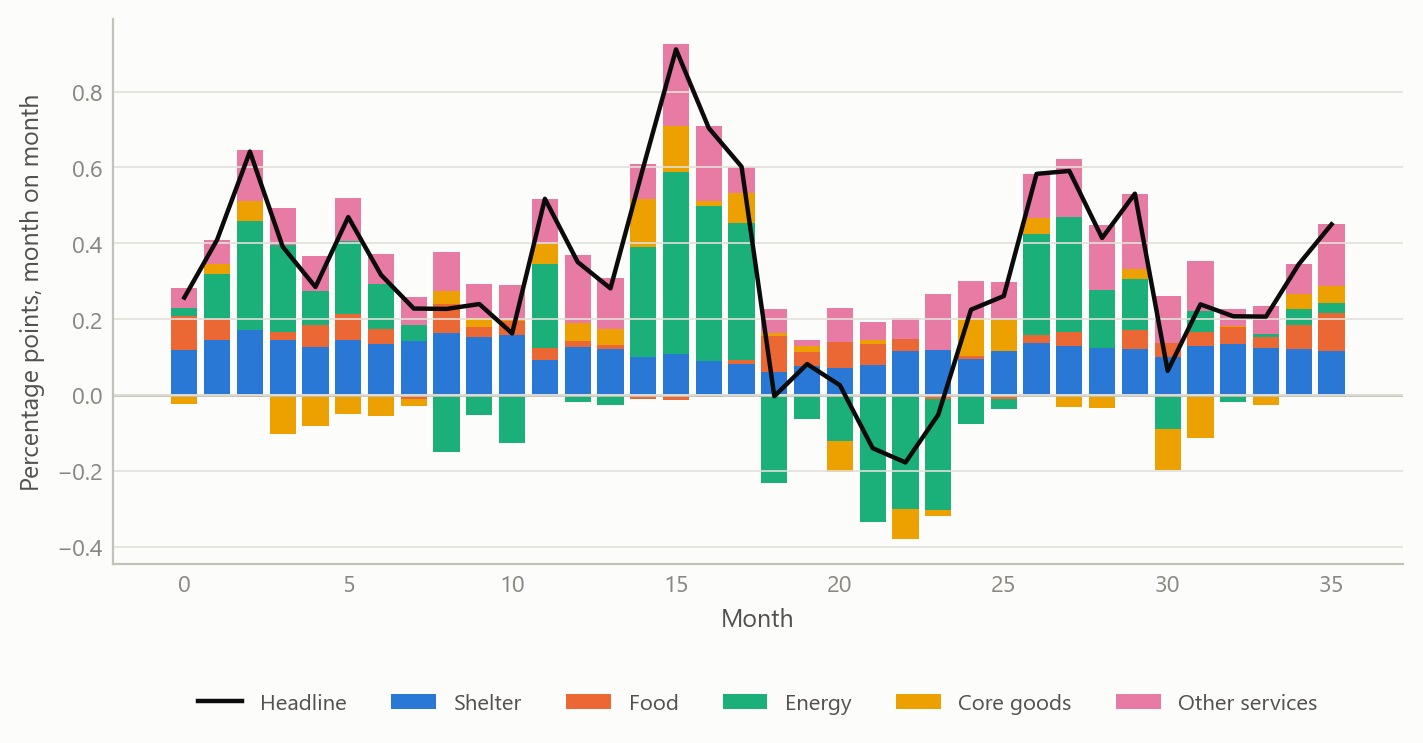
\includegraphics[keepaspectratio]{index_files/figure-latex/fig-contrib-output-1.png}}

}

\caption{\label{fig-contrib}Monthly contributions to headline inflation
by major group, with the headline change as a line (simulated data).}

\end{figure}%

The picture is the one a forecaster wants. A large swing in energy
dominates the headline for a few months, while shelter contributes a
steady positive amount that changes slowly. The routine delivers this
view for every group and every lower-level component, and a month's
surprise can be traced to the few components that produced it.

\subsubsection{Weights that move within the
year}\label{weights-that-move-within-the-year}

Holding weights fixed until the next December would be simpler, but it
lets the decomposition drift away from the headline. Rolling the weights
forward each month keeps each component's share current. A component
with fast price growth gains share through the year and is then reset
when new annual weights arrive.

\begin{figure}

\centering{

\pandocbounded{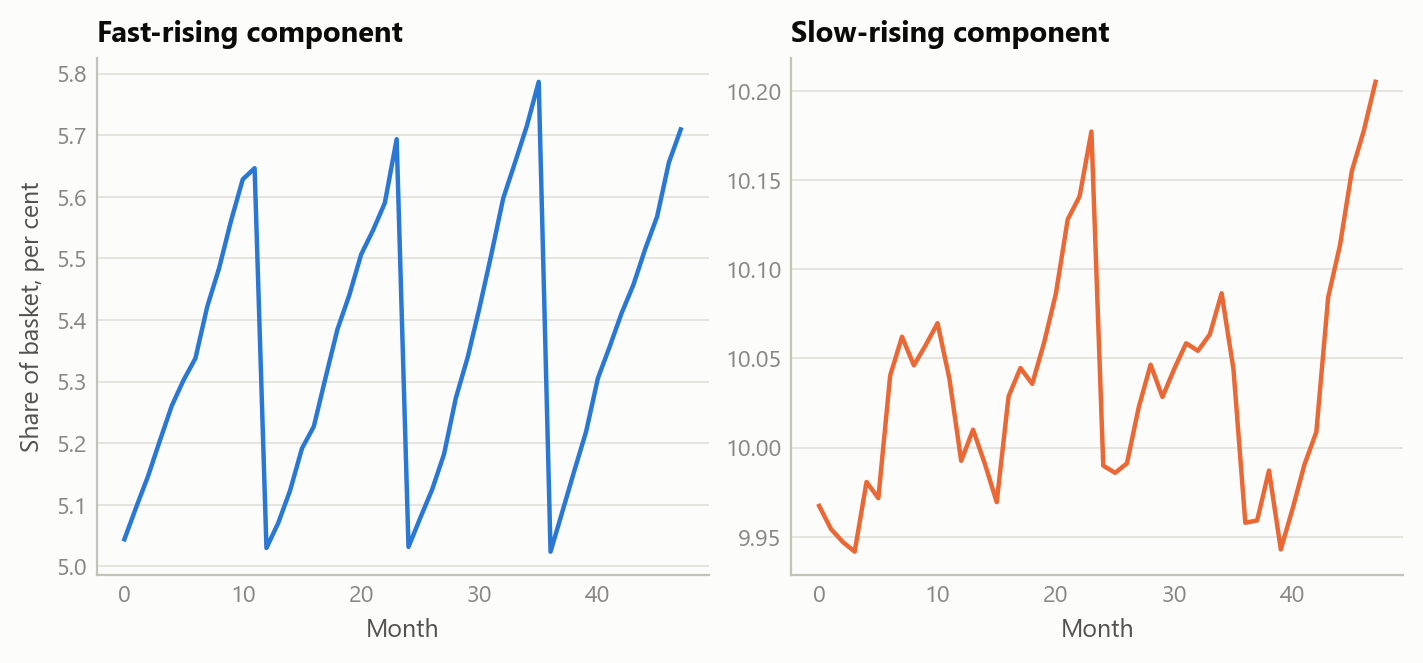
\includegraphics[keepaspectratio]{index_files/figure-latex/fig-weights-output-1.png}}

}

\caption{\label{fig-weights}Effective weight of a fast-rising and a
slow-rising component, rolled forward within each year and reset each
December (simulated data).}

\end{figure}%

\subsubsection{Extending back before the machine-readable
weights}\label{extending-back-before-the-machine-readable-weights}

Machine-readable annual weights were available only from 2011. For 2006
to 2010 the weights existed as December text tables without series
codes. They were matched to the component catalogue by name, and 175 of
183 series, or 95.6 per cent, could be matched. The unmatched components
were traced; they were series that already existed in 2006, and they
were flagged for synonym mappings. A first match summed to about twice
the expected total because aggregates and their parts had both been
matched, which is why the final construction keeps only the lowest-level
leaves and rescales them to sum to one hundred. The resulting weight
vintages then run through the same monthly engine, so the early years
splice onto the later ones without a break in method.

\begin{figure}

\centering{

\pandocbounded{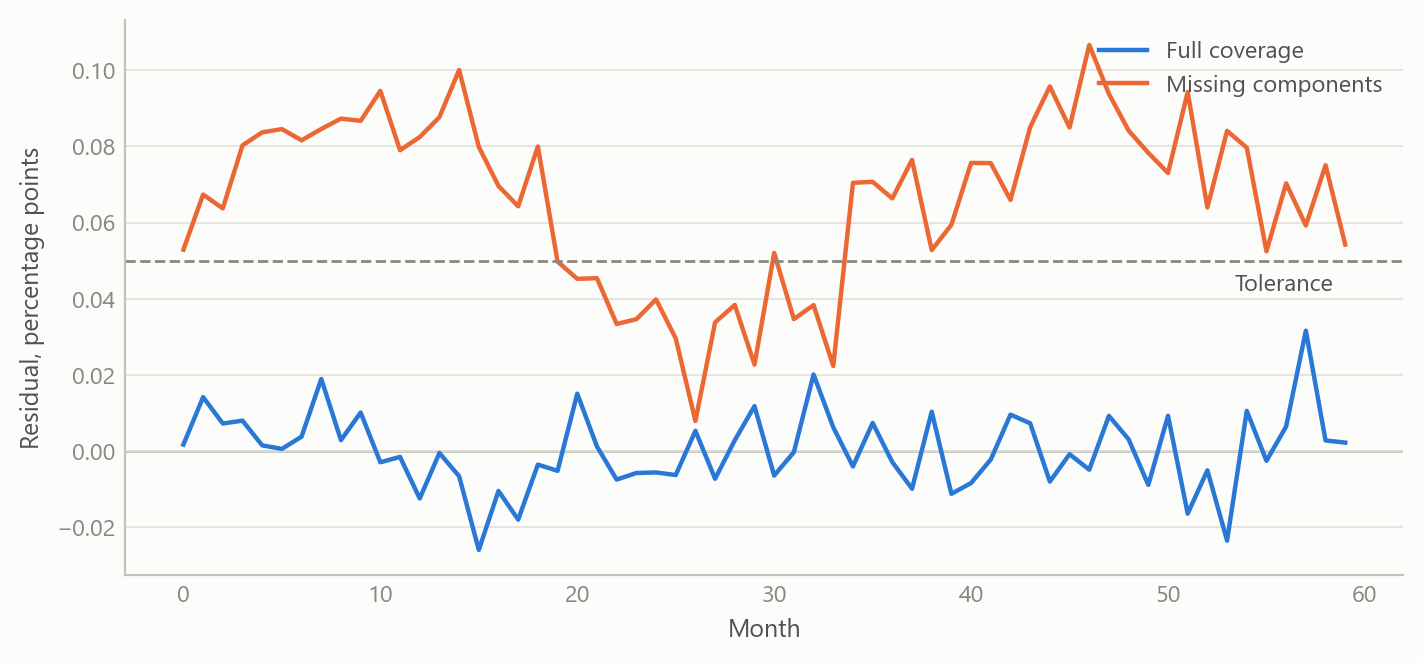
\includegraphics[keepaspectratio]{index_files/figure-latex/fig-resid-output-1.png}}

}

\caption{\label{fig-resid}Residual between headline and summed
contributions, with full and with incomplete component coverage
(simulated data).}

\end{figure}%

The residual is the feed's smoke alarm. With complete coverage it is
close to zero, as the first line shows. When components are missing it
leans away from zero, which is how coverage gaps announce themselves.

\subsection{Insights}\label{insights}

\begin{itemize}
\tightlist
\item
  \textbf{Build the check into the pipeline.} Storing the reconciliation
  residual every month turns a hidden assumption into a monitored
  quantity. Problems with coverage, hierarchy or weights show up as a
  pattern that can be diagnosed.
\item
  \textbf{Refuse partial data.} An update that fails loudly and leaves
  the base unchanged is better than one that writes a dataset with gaps.
  Downstream models cannot tell a hole from a real zero.
\item
  \textbf{Revisions are part of the data.} A refresh that only appends
  new months would keep stale values. A rolling window that overwrites
  recent months, wider early in the year, keeps the stored history
  current.
\item
  \textbf{Check before you fetch.} A sentinel query avoids the cost of a
  full pull when nothing has been published, which respects the
  provider's limits and makes scheduling cheap.
\item
  \textbf{Match on structure first, names second.} Name matching worked
  for most components but needed leaf filtering and a handful of manual
  synonyms. Prior structure in the codes carried most of the load.
\end{itemize}

\subsection{Limits and next steps}\label{limits-and-next-steps}

The feed is a data layer, not a forecast. It does not show forecast
accuracy, and nothing here claims that the decomposition improves
predictions of inflation. The simulated figures illustrate the
construction; they are not results.

Several limits are known. The reconstructed weights are an approximation
based on prior-month prices, so small residuals are expected even with
full coverage. The weights for 2006 to 2010 depend on name matching,
with a small set of unmatched components still awaiting mapping. The
feed covers the all-urban-consumers index only, so other price measures
would need their own mappings.

The next steps are a union of all weight vintages for fuller historical
coverage, a decomposition of the residual into coverage and rounding
parts, and linking the contributions to component-level forecasting
models so that the bottom-up and top-down views can be compared out of
sample.

\subsection{About the evidence}\label{about-the-evidence}

The work was carried out in 2025 on monthly US consumer price data from
January 2006 onward. The statements about the feed's design, the
175-of-183 name match and the weight construction come from the
project's own documentation and outputs. All figures here use simulated
data with the same structure, and the numbers in them are illustrative.

Figures and tables marked \emph{simulated} are generated from simulated
data built to share the structure of the analysis (its variables,
horizons and frequencies). They show how the method works and what its
output looks like; they are not the project's results. Results stated in
the text are the project's own. Methods are described at the level of a
methods section. Code and data pipelines are not reproduced here.




\end{document}
